%!TEX root = ../main.tex
\section{Deep Neural Networksの基礎}
\subsection{なぜいまAIブームなのか}
現在、第3期AIブームだといわれる。第1期は1956年に開催されたダートマス会議を契機として1970年前半まで続いたもので、パーセプトロンの原理が発明され、数学定理の証明や言語意味理解などが試みられた。第2期は1980年台に起こり、Multi Layer Perceptron (MLP)を効率よく学習させるBack Probagation (BP)手法が確立されたほか、ある専門領域の知識を何らかの形で抽出し質問に答えたり問題を解いたりするエキスパートシステム研究が盛んに行われた。国内でも第五世代コンピュータの研究開発プロジェクトに莫大な資金が投入された。しかし、いずれのブームも大きな失望感とともに急速に廃れ、とある国際会議ではArtificial Intelligenceというキーワードが入っているだけで論文が落とされるというジョークもまことしやかにささやかれるほどであった。

では、いまなぜ改めて第3期AIブームなのだろうか?現在のAIブームを牽引しているのはDeep Neural Networks (DNN, 深層学習)であることは間違いない。しかし、現在のDNNの源流となるネオコグニトロンは1980年前後にすでに(当時NHK放送技術研究所の)福島ら\cite{fukushima79,fukushima80,fukushima83}によって提案されている。原因は諸説あるが、下記のような複数の技術的要因がうまく噛み合ったためだと思わる。
\begin{itemize}
\item SNSの流行、IoT技術の普及などにより様々なドメインのデータがビッグデータ化した。
\item GPUやクラウドコンピュータなどDNNを現実的な時間内で計算終了できるだけの計算資源が得られるようになった。
\item クラウドワーキングによって正解データを作成してくれる人の確保が格段に容易になった。
\end{itemize}
特にDNNをうまく動作させようと思うと、学習のための膨大なデータが必要である。Weakly-supervised Learning (弱教師学習)やSemi-supervised Learning (半教師付き学習)など全てのトレーニングデータに正解を付与しなくともある程度学習ができるようになるアルゴリズムは存在するが、それは正解が得られない場合の回避策であり、全てのトレーニングデータに対して正解が付与されている状態が最大の性能を発揮する。半導体の講義で学習したであろうムーアの法則に則って考えると、計算機は3年で4倍の性能を得ることができるので30年前と比べてざっと100万倍の計算能力を手に入れた計算になる。これは、現在1日かけて行う計算は30年前の計算機では100万日かかっていたことを意味するが、30年前から今日まで1万日ちょっとしか経っていない。

さらには、社会的な情勢もそれを後押ししたと指摘する研究者もいる。
\begin{itemize}
\item Google, Facebook, Microsoftなど巨大IT企業がDNNを重要視し、それぞれTensorFlow, PyTorch, The Microsoft Cognitive Toolkit (CNTK)などのディープラーニングフレームワーク(ソフトウェアライブラリ)を作成・公開した。また、国内でもPFN社がChainerを公開。
\item オープンソース化が主流となり、GitHubなど多くのプラットフォームを利用して団体や個人が作成したソフトウェアが公開去れるようになった。これにより、自分で実装をする必要がなくなり、すぐに試せる、もしくは公開されている機能から先のみを実装すればよくなった。
\item 論文もオープンソース化の流れにのり、多くの出版社でオープンソースとして公開去れることが増えた。また、ArXivのように速報性を重視するサービスも登場し、その流れを一層加速させた。
\item 物体認識コンテストのように、多くのコンテストが開催され、同じデータで多くの研究者が競い、性能の差異が議論しやすくなった。また、Kaggleのようにコンテスト・ランキングをビジネスにするサービスも現れた。
\end{itemize}
学生の諸君は信じられないであろうが、ほんの10-20年前は画像を読み込むにも自前で実装するところから始めなくてはならなかった。そのため、ソフトウェアの開発効率は今と比べて極めて悪かったのである。いまはArXivにいち早く一流国際会議に投稿された会議が掲載され(当落の保証はない)、ソースコードとデータセットが同時に公開され、それらをDLすれば一瞬で再現でき、しかも前述のフレームワークの登場で可読性が極めて高く改変がやりやすい。という時代である。Twitterやブログで一気に話題化するのも要因の一つであろう。



\subsection{人工知能, 機械学習, 深層学習}
人工知能, 機械学習, 深層学習が同列に語られることも多いが、厳密に言うと機械学習は人工知能技術の1つであり、深層学習は機械学習技術の1手法という位置づけである。特にマスコミの記事などでは受けの良さから「人工知能による処理」と謳うものが多くなりがちであるが、必ずしもそれは学習ベースの処理出ないこともあるので注意が必要である。

\begin{figure}[ht]
	\begin{center}
		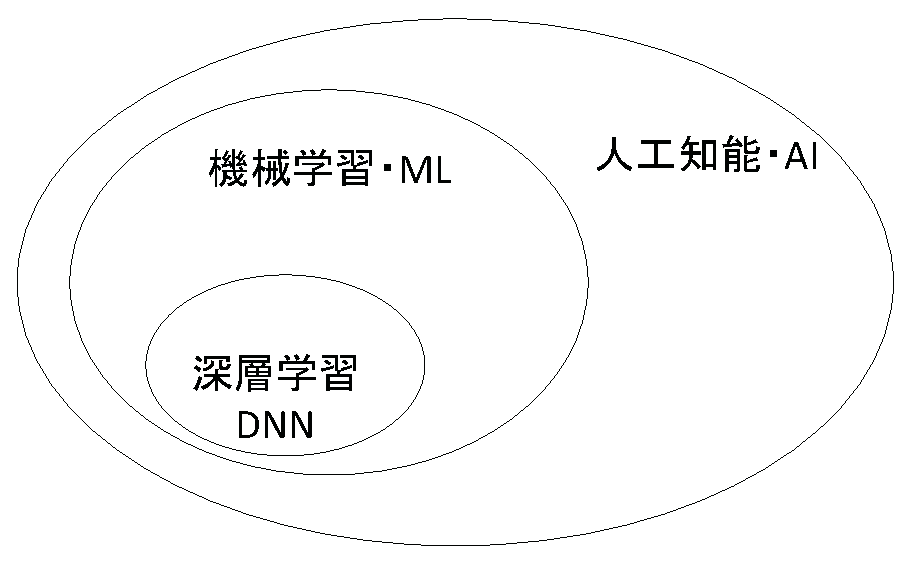
\includegraphics[width=0.7\linewidth] {images/YamasakiLab/introduction/AI_ML_DNN.eps}
		\caption{人工知能、機械学習、深層学習の関係。}
		\label{fig:accuracy}
	\end{center}
\end{figure}


\subsection{DNNは何が破壊的だったか?}
画像認識を例に、果物の画像を分類するシステムを開発すると仮定しよう。りんごとみかんとバナナ・・・を認識しようとしたとき、自分でプログラムを書くとしたら何を手がかりとしてそれらの画像を分類するだろうか?赤ければりんご、橙色であればみかん、黄色であればバナナ・・・としてみればどうだろう。しかし、これは例えば青りんごや未完熟の緑色の果実はうまく分類することができない。それでは、大きな丸い形はりんご、小さい楕円形はみかん、長細ければバナナ・・・としてみてはどうだろう。と、このように複数のクラスをうまく切り分けることのできる画像特徴を考えるのが一般的である。DNN以前の画像認識はまさにこの例に述べた通り画像認識に有効な新しい特徴を人間が考えるというのが画像認識の研究だった。特徴ベクトルを一旦抽出することができればあとはSuport Vector Machine (SVM)やRandom Forest (RF)など成熟した既存の機械学習器を用いて実際の認識・分類を行う。

DNNを用いた画像認識では、DNNに与えるのは画像そのものと正解ラベルのみである。画像を分類するための特徴はDNNが自動で考えるのである。言葉で記述するとそれだけなのであるが、人間が特徴を考えるよりも効率的な特徴設計ができる。画像分類ではILSVRCという1000クラスの画像を分類する国際コンテストが行われている。DNN以前は何らかの工夫により毎年1~2\%ずつ誤差率が下がっていくというのが一般的であったが、2012年にDNNが初めて用いられたときには人間が考えた特徴量による最高性能が誤差率26\%であったのに対し、DNNの誤差率は15\%と、実に10\%以上もの差をつけて大勝した。その後、DNNは音声やタンパク質の結合予測コンテストでも軒並みこれまでの「人間が考える特徴量」に大差をつけて優勝し、DNN大流行のきっかけとなった。

もちろん、DNNの登場によってやることはなくなったかというとそうではない。DNNは深層学習の一般的な呼称であり、どのようなネットワークを構築するかは利用者の手に委ねられている。また、学習に関わる様々なハイパーパラメータなども人間が決定しなければならない。

\begin{figure}[ht]
	\begin{center}
		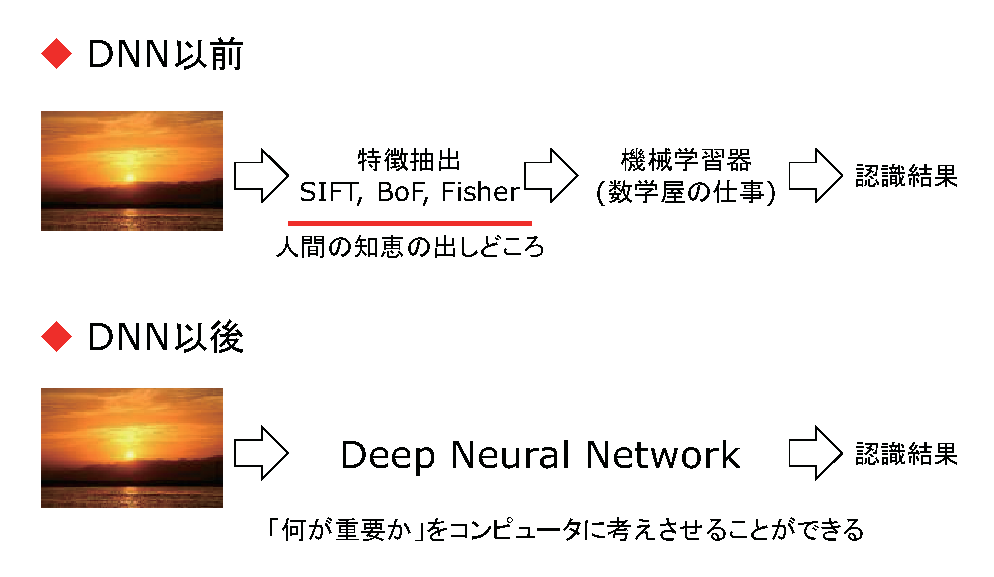
\includegraphics[width=0.7\linewidth] {images/YamasakiLab/introduction/before_after_dnn.eps}
		\caption{DNN以前とDNN以後の画像認識手法の違い。}
		\label{fig:accuracy}
	\end{center}
\end{figure}

\subsection{DNNの特徴}
上記に述べた通り、特徴の設計も自動的にできるという利点以外に、下記にあげるような利点・特徴がある。

\subsubsection{バッチ型ではなく逐次型の学習である}
Support Vector Machine (SVM), Random Forest (RF)を始め、主要な機械学習技術の殆どがバッチ型学習、すなわち学習データはすべてそろえたあとすべてを一気に使って学習させるという手法をとる。そのほうが学習データの分布を見渡した上で最適な学習が行えるためである。SVMやRFを逐次学習、すなわち少しずつ学習データが増えていった場合に対応去せる試みもなされてきたがバッチ学習と比べると精度は遠く及ばないものであった。

それに対して、NNは学習データを少量ずつ見ては内部のパラメータを更新していくという手法をとる。もちろん、初期のパーセプトロンでは学習データ1つごとにパラメータ更新を行っていたが、それではBPを行った際ノイズに弱くなるので現在のDNNでは複数の学習データに対する誤差を平均化してBPする手法(ミニバッチ)など工夫はなされている。逐次学習は裏を返せば学習を途中で止めて、その後ネットワーク構造や学習データを変化させて学習を続けても良いということを示しており、この特徴が下記に続く様々な特徴へと続いていく。


\subsubsection{Transfer learning (転移学習)が容易である}
対象とするクラスの教師画像が多数無い場合が存在する。最初大量にトレーニング画像を準備できるクラスでpre-trainしたあと対象クラス画像でfine-tuneすると高性能が出ることが知られている。例えて言えば、果物の分類器と花の分類器があったとする。果物の画像は集めるのが容易だが花の画像を集めるのは困難であるとしよう。これまでは、果物の分類器と花の分類器は独立して学習しなければならず、果物の分類器を花の分類に転用するのは困難な問題であった。そのため、花の分類性能を向上させるためには花のトレーニングデータの数を増やすしかなかった。

しかし、DNNでは
\begin{itemize}
\item ある程度画像認識一般に有用な汎用的な特徴表現を内部表現として獲得している
\item 逐次学習であるため、途中からトレーニングデータを変えても学習を進められる
\end{itemize}
などの特徴があるためである。この特徴のお陰で様々な分野へ画像分類の応用が可能となった。ただし、闇雲にデータを集めても転移学習がうまくいくわけでなく、画像の種類が大きく異なるような場合は転移学習の効果が得られにくくスクラッチ学習(他のデータを使わないで0から学習)したほうが性能が高い場合もあるので注意が必要である。また、そのような問題に対して研究するCross-Domain Learning (ドメインを跨ぐ学習)という研究領域も存在する。



\subsubsection{ネットワークの分岐が容易である}
Neural Networkは文字通りネットワークであるため、途中で分岐させることが容易である。これが、DNNの性能を向上させる要因の一つとなっている。

\subsubsubsection{ネットワークが途中で複数に分離する場合}
途中までのネットワーク構造を共通にして、途中から複数に分離し、複数のタスクを解くネットワークを学習させることができる。これをMulti-task Learningと呼ぶ。前段の共通ネットワークは、複数のタスクからの誤差率が逆伝搬されパラメータがアップデートされる。すなわち、前段ネットワークは複数タスクを同時に解くのに効率的なネットワークになっていることが期待される。

\subsubsubsection{ネットワークが途中で1つに集約する場合}
複数のネットワークに異なるモーダルのデータを入力し、途中で1つのネットワークに統合してタスクを解くネットワークを学習させることができる。これをMulti-feature Fusionと呼ぶ。これまでの機械学習では、画像、音声、テキストなどモーダルの異なるデータを融合して総合的に学習を行うことが困難であった。しかし、このネットワーク構造では複数種類のデータをどのように結合すればよいかについてもDNNが自動的に最適化するので無理のないMulti-feature Fusionが可能となる。

\begin{figure}[ht]
	\begin{center}
		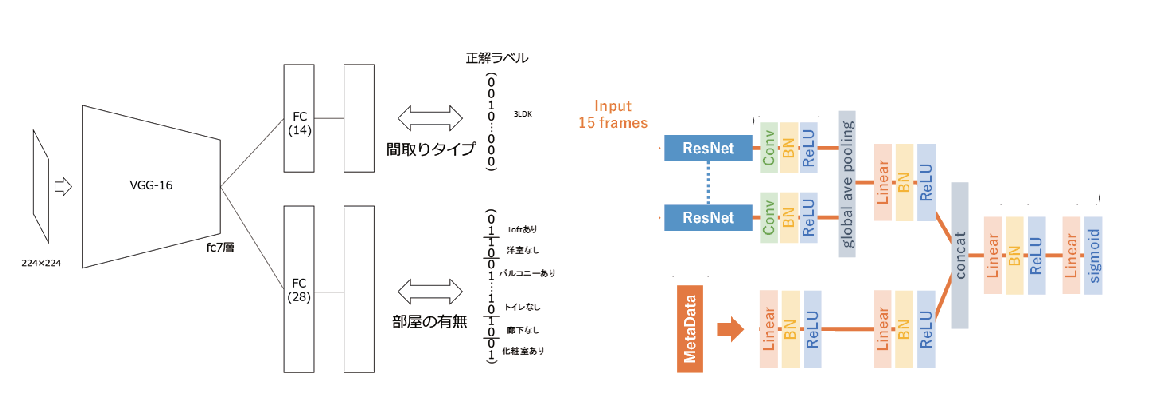
\includegraphics[width=0.7\linewidth] {images/YamasakiLab/introduction/branch.eps}
		\caption{ネットワークの分岐。(左) Multi-task Learning、(右) Multi-feature Fusion。}
		\label{fig:accuracy}
	\end{center}
\end{figure}

\subsubsection{データのモーダル間の垣根が少なくなった}
本実験ではたった10日間の日程で画像・音声・言語を対象としている。一昔まえであればそれぞれ10日間のプログラムにしてもおかしくないほど異なる専門知識が必要とされたきた。しかし、DNNによって画像・音声・言語といったモーダルの違いは以前に比べて意識しなくても良くなってきている。それぞれのモーダルに応じてちょっとした前処理に違いは生じるものの、一旦DNNの中に入力してしまえば、もしくはDNN特徴量として表現してしまえば、それらのデータの扱いは全く同じになる。それを証拠に、現在image2text, text2imageといった画像と言語の融合や、「猫」という画像表現と「猫」の鳴き声が特徴空間では互いに近くなるよう学習する手法などが登場している。

\subsection{Neural Network基礎}
山崎の講義を参照すること。


